%%
%% Copyright 2007, 2008, 2009 Elsevier Ltd
%%
%% This file is part of the 'Elsarticle Bundle'.
%% ---------------------------------------------
%%
%% It may be distributed under the conditions of the LaTeX Project Public
%% License, either version 1.2 of this license or (at your option) any
%% later version.  The latest version of this license is in
%%    http://www.latex-project.org/lppl.txt
%% and version 1.2 or later is part of all distributions of LaTeX
%% version 1999/12/01 or later.
%%
%% The list of all files belonging to the 'Elsarticle Bundle' is
%% given in the file `manifest.txt'.
%%
\documentclass[3p,authoryear,preprint,12pt]{elsarticle}
\makeatletter\if@twocolumn\PassOptionsToPackage{switch}{lineno}\else\fi\makeatother

      \makeatletter
\usepackage{wrapfig}
\newcounter{aubio}

\long\def\bioItem{%
\@ifnextchar[{\@bioItem}{\@@bioItem}}

\long\def\@bioItem[#1]#2#3{
 \stepcounter{aubio}
 \expandafter\gdef\csname authorImage\theaubio\endcsname{#1}
 \expandafter\gdef\csname authorName\theaubio\endcsname{#2}
 \expandafter\gdef\csname authorDetails\theaubio\endcsname{#3}
}

\long\def\@@bioItem#1#2{
 \stepcounter{aubio}
 \expandafter\gdef\csname authorName\theaubio\endcsname{#1}
 \expandafter\gdef\csname authorDetails\theaubio\endcsname{#2}
}

\newcommand{\checkheight}[1]{%
  \par \penalty-100\begingroup%
  \setbox8=\hbox{#1}%
  \setlength{\dimen@}{\ht8}%
  \dimen@ii\pagegoal \advance\dimen@ii-\pagetotal
  \ifdim \dimen@>\dimen@ii
    \break
  \fi\endgroup}

\def\printBio{%
  \@tempcnta=0
   \loop
     \advance \@tempcnta by 1
     \def\aubioCnt{\the\@tempcnta}
     \setlength{\intextsep}{0pt}%
     \setlength{\columnsep}{10pt}%
     \newbox\boxa%
     \setbox\boxa\vbox{\csname authorDetails\aubioCnt\endcsname}
     \expandafter\ifx\csname authorImage\aubioCnt\endcsname\relax%
      \else%
       \checkheight{\includegraphics[height=1.25in,width=1in,keepaspectratio]{\csname authorImage\aubioCnt\endcsname}}
        \begin{wrapfigure}{l}{25mm}
         \includegraphics[height=1.25in,width=1in,keepaspectratio]{\csname authorImage\aubioCnt\endcsname}%height=145pt
        \end{wrapfigure}\par
      \fi
     {\parindent0pt\textbf{\csname authorName\aubioCnt\endcsname}\csname authorDetails\aubioCnt\endcsname \par\bigskip%
     \expandafter\ifx\csname authorImage\aubioCnt\endcsname\relax\else%
      \ifdim\the\ht\boxa < 90pt\vskip\dimexpr(90pt -\the\ht\boxa-1pc)\fi%
     \fi}%for adding additional vskip for avoiding image overlap.
      \ifnum\@tempcnta < \theaubio
   \repeat
   }

\makeatother

      

\usepackage{tabulary,xcolor}
\usepackage{amsfonts,amsmath,amssymb}
\usepackage[T1]{fontenc}
\makeatletter
\let\save@ps@pprintTitle\ps@pprintTitle
\def\ps@pprintTitle{\save@ps@pprintTitle\gdef\@oddfoot{\footnotesize\itshape \null\hfill\today}}
\def\hlinewd#1{%
  \noalign{\ifnum0=`}\fi\hrule \@height #1%
  \futurelet\reserved@a\@xhline}
\def\tbltoprule{\hlinewd{.8pt}\\[-12pt]}
\def\tblbottomrule{\noalign{\vspace*{6pt}}\hline\noalign{\vspace*{2pt}}}
\def\tblmidrule{\noalign{\vspace*{6pt}}\hline\noalign{\vspace*{2pt}}}
\AtBeginDocument{\ifNAT@numbers \biboptions{sort&compress}\fi}
\makeatother

  


\usepackage{ifluatex}
\ifluatex
\usepackage{fontspec}
\defaultfontfeatures{Ligatures=TeX}
\usepackage[]{unicode-math}
\unimathsetup{math-style=TeX}
\else 
\usepackage[utf8]{inputenc}
\fi 
\ifluatex\else\usepackage{stmaryrd}\fi

  
%%%%%%%%%%%%%%%%%%%%%%%%%%%%%%%%%%%%%%%%%%%%%%%%%%%%%%%%%%%%%%%%%%%%%%%%%%
% Following additional macros are required to function some 
% functions which are not available in the class used.
%%%%%%%%%%%%%%%%%%%%%%%%%%%%%%%%%%%%%%%%%%%%%%%%%%%%%%%%%%%%%%%%%%%%%%%%%%
\usepackage{url,multirow,morefloats,floatflt,cancel,tfrupee}
\makeatletter


\AtBeginDocument{\@ifpackageloaded{textcomp}{}{\usepackage{textcomp}}}
\makeatother
\usepackage{colortbl}
\usepackage{xcolor}
\usepackage{pifont}
\usepackage[nointegrals]{wasysym}
\urlstyle{rm}
\makeatletter

%%%For Table column width calculation.
\def\mcWidth#1{\csname TY@F#1\endcsname+\tabcolsep}

%%Hacking center and right align for table
\def\cAlignHack{\rightskip\@flushglue\leftskip\@flushglue\parindent\z@\parfillskip\z@skip}
\def\rAlignHack{\rightskip\z@skip\leftskip\@flushglue \parindent\z@\parfillskip\z@skip}

%Etal definition in references
\@ifundefined{etal}{\def\etal{\textit{et~al}}}{}


%\if@twocolumn\usepackage{dblfloatfix}\fi
\usepackage{ifxetex}
\ifxetex\else\if@twocolumn\@ifpackageloaded{stfloats}{}{\usepackage{dblfloatfix}}\fi\fi

\AtBeginDocument{
\expandafter\ifx\csname eqalign\endcsname\relax
\def\eqalign#1{\null\vcenter{\def\\{\cr}\openup\jot\m@th
  \ialign{\strut$\displaystyle{##}$\hfil&$\displaystyle{{}##}$\hfil
      \crcr#1\crcr}}\,}
\fi
}

%For fixing hardfail when unicode letters appear inside table with endfloat
\AtBeginDocument{%
  \@ifpackageloaded{endfloat}%
   {\renewcommand\efloat@iwrite[1]{\immediate\expandafter\protected@write\csname efloat@post#1\endcsname{}}}{\newif\ifefloat@tables}%
}%

\def\BreakURLText#1{\@tfor\brk@tempa:=#1\do{\brk@tempa\hskip0pt}}
\let\lt=<
\let\gt=>
\def\processVert{\ifmmode|\else\textbar\fi}
\let\processvert\processVert

\@ifundefined{subparagraph}{
\def\subparagraph{\@startsection{paragraph}{5}{2\parindent}{0ex plus 0.1ex minus 0.1ex}%
{0ex}{\normalfont\small\itshape}}%
}{}

% These are now gobbled, so won't appear in the PDF.
\newcommand\role[1]{\unskip}
\newcommand\aucollab[1]{\unskip}
  
\@ifundefined{tsGraphicsScaleX}{\gdef\tsGraphicsScaleX{1}}{}
\@ifundefined{tsGraphicsScaleY}{\gdef\tsGraphicsScaleY{.9}}{}
% To automatically resize figures to fit inside the text area
\def\checkGraphicsWidth{\ifdim\Gin@nat@width>\linewidth
	\tsGraphicsScaleX\linewidth\else\Gin@nat@width\fi}

\def\checkGraphicsHeight{\ifdim\Gin@nat@height>.9\textheight
	\tsGraphicsScaleY\textheight\else\Gin@nat@height\fi}

\def\fixFloatSize#1{}%\@ifundefined{processdelayedfloats}{\setbox0=\hbox{\includegraphics{#1}}\ifnum\wd0<\columnwidth\relax\renewenvironment{figure*}{\begin{figure}}{\end{figure}}\fi}{}}
\let\ts@includegraphics\includegraphics

\def\inlinegraphic[#1]#2{{\edef\@tempa{#1}\edef\baseline@shift{\ifx\@tempa\@empty0\else#1\fi}\edef\tempZ{\the\numexpr(\numexpr(\baseline@shift*\f@size/100))}\protect\raisebox{\tempZ pt}{\ts@includegraphics{#2}}}}

%\renewcommand{\includegraphics}[1]{\ts@includegraphics[width=\checkGraphicsWidth]{#1}}
\AtBeginDocument{\def\includegraphics{\@ifnextchar[{\ts@includegraphics}{\ts@includegraphics[width=\checkGraphicsWidth,height=\checkGraphicsHeight,keepaspectratio]}}}

\DeclareMathAlphabet{\mathpzc}{OT1}{pzc}{m}{it}

\def\URL#1#2{\@ifundefined{href}{#2}{\href{#1}{#2}}}

%%For url break
\def\UrlOrds{\do\*\do\-\do\~\do\'\do\"\do\-}%
\g@addto@macro{\UrlBreaks}{\UrlOrds}



\edef\fntEncoding{\f@encoding}
\def\EUoneEnc{EU1}
\makeatother
\def\floatpagefraction{0.8} 
\def\dblfloatpagefraction{0.8}
\def\style#1#2{#2}
\def\xxxguillemotleft{\fontencoding{T1}\selectfont\guillemotleft}
\def\xxxguillemotright{\fontencoding{T1}\selectfont\guillemotright}

\newif\ifmultipleabstract\multipleabstractfalse%
\newenvironment{typesetAbstractGroup}{}{}%

%%%%%%%%%%%%%%%%%%%%%%%%%%%%%%%%%%%%%%%%%%%%%%%%%%%%%%%%%%%%%%%%%%%%%%%%%%
\emergencystretch 20pt \tolerance = 1500 \def\floatpagefraction{0.8}




\begin{document}



\begin{frontmatter}
	
\title{Roaming Around AML
}
    
\author[abb6a21433054]{Reza Asakereh}
\ead{rasakereh@ce.sharif.edu}
    
\address[abb6a21433054]{CE Department\unskip, 
    Sharif University of Technology}
  

\begin{abstract}
 AML is a lethal type of blood cancer originating from bone marrow. This article is devoted to analyze microarray data and derive a number of differentially expressed genes, consequently to come up with a handful of information. An immune system interaction with AML in the form of both cause and effect is once again verified. 
\end{abstract}
\end{frontmatter}
    
\section{Introduction}
 This article conducts an unplanned investigation of bunch of data and research results about AML decease. As indicated by \cite{doi:10.3322/canjclin.55.2.74}, the fifth most affected site in body by cancer is the circulatory system, with about a hundred thousands estimated cases in total of a million cancer in the US, 2002. AML is one of the most suffered and fatal one with almost 35\% of the cases resulting into death. Hence, piling up some results in this area will accelerate more experienced scientists toward a working solution. However, this field is not abandoned, and has been worked on extensively. Therefore, they are considered as rich sources of result validation. The process of the investigation begins with a beginner level differential expression analysis resulting in some gene lists with significant gene expression alterations. These lists are used as the input of the next pipeline component, gene enrichment. Extracting some pieces of information in this step will be the basis of some fact finding endeavors.

\section{Data Preparation and Validation}
The data can be accessed via GSE48558 accession number. Primarily, to verify if data is normalized and the comparisons are mathematically meaningful, a box plot was employed, resulting in Figure 1.
\bgroup
\fixFloatSize{img/boxplot.png}
\begin{figure*}[!htbp]
	\centering \makeatletter\IfFileExists{img/boxplot.png}{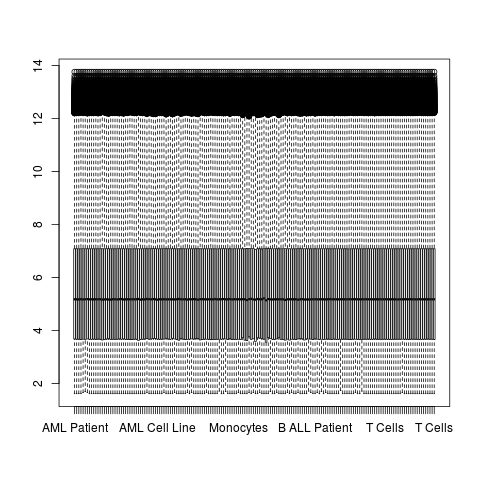
\includegraphics{img/boxplot.png}}{}
	\makeatother 
	\caption{{The data needs no additional normalization.}}
	\label{f-c2b15a1baca9}
\end{figure*}
\egroup

As the data needed no preprocessing, the process of validation was embarked on, which indicated a great clustering and reliability of B Cell data in comparison with other data subgroups. Figure 2 to Figure 10 would depict the claim.

\bgroup
\fixFloatSize{img/mixHeatmap.png}
\begin{figure*}[!htbp]
	\centering \makeatletter\IfFileExists{img/mixHeatmap.png}{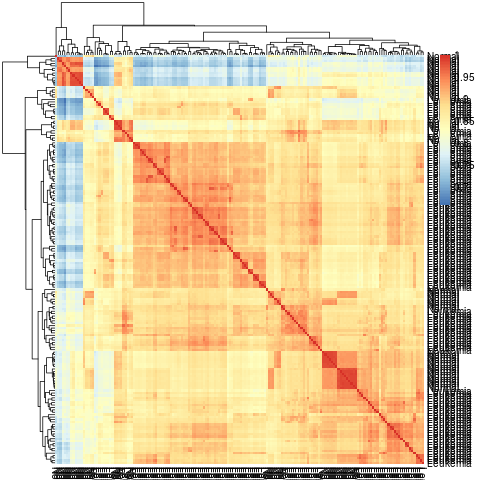
\includegraphics{img/mixHeatmap.png}}{}
	\makeatother 
	\caption{{The heat map for the mixture of cells, showing poor clustering. Clustering score was not calculated due to the god damn deadline.}}
	\label{f-c2b15a1bacb9}
\end{figure*}
\egroup
\bgroup
\fixFloatSize{img/THeatmap.png}
\begin{figure*}[!htbp]
	\centering \makeatletter\IfFileExists{img/THeatmap.png}{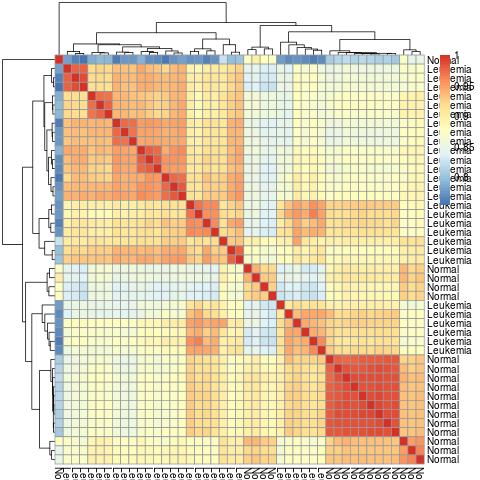
\includegraphics{img/THeatmap.png}}{}
	\makeatother 
	\caption{{The heat map for T cells, showing relatively better clustering. Clustering score was not calculated due to the god damn deadline.}}
	\label{f-c2b15a1bacc9}
\end{figure*}
\egroup
\bgroup
\fixFloatSize{img/BHeatmap.png}
\begin{figure*}[!htbp]
	\centering \makeatletter\IfFileExists{img/BHeatmap.png}{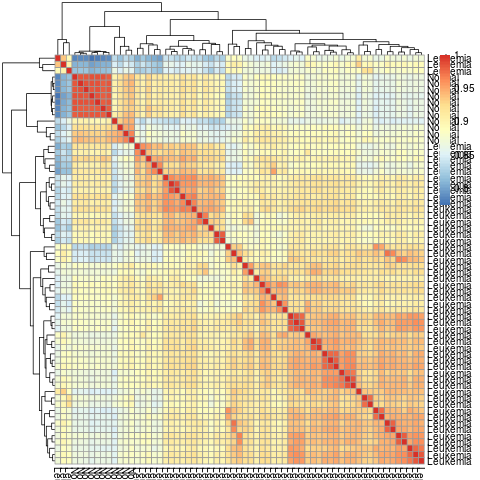
\includegraphics{img/BHeatmap.png}}{}
	\makeatother 
	\caption{{The heat map for the B cells, showing almost perfect clustering. Clustering score was not calculated due to the god damn deadline.}}
	\label{f-c2b15a1bacd9}
\end{figure*}
\egroup

In addition to the clustering property, separability was assessed using two dimension reduction mechanisms, PCA and t-SNE.

\bgroup
\fixFloatSize{img/mixPCA.png}
\begin{figure*}[!htbp]
	\centering \makeatletter\IfFileExists{img/mixPCA.png}{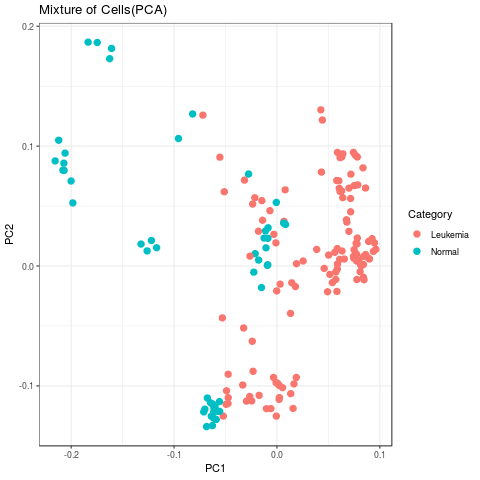
\includegraphics{img/mixPCA.png}}{}
	\makeatother 
	\caption{{PCA indicates poor separability in cell mixture.}}
	\label{f-c2b15a1bace9}
\end{figure*}
\egroup
\bgroup
\fixFloatSize{img/TPCA.png}
\begin{figure*}[!htbp]
	\centering \makeatletter\IfFileExists{img/TPCA.png}{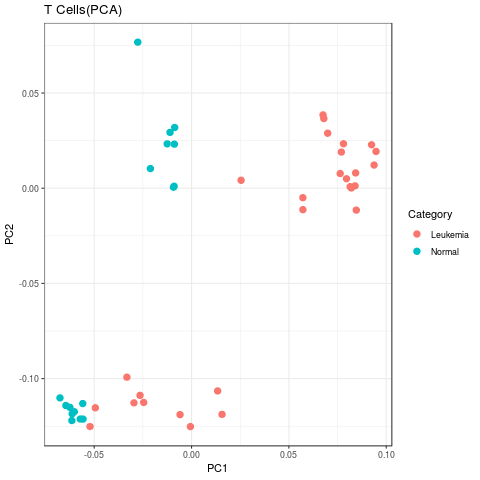
\includegraphics{img/TPCA.png}}{}
	\makeatother 
	\caption{{PCA indicates relatively better separability in T cells.}}
	\label{f-c2b15a1bacf9}
\end{figure*}
\egroup
\bgroup
\fixFloatSize{img/BPCA.png}
\begin{figure*}[!htbp]
	\centering \makeatletter\IfFileExists{img/BPCA.png}{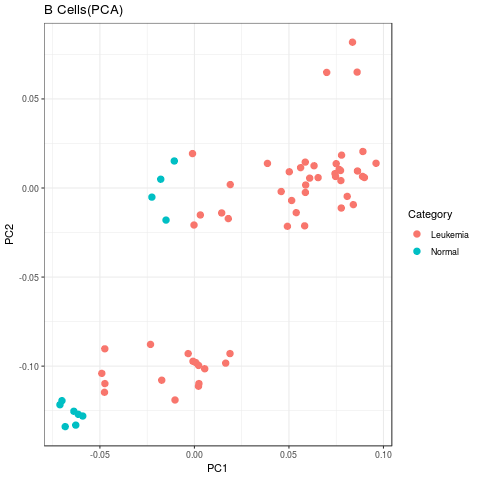
\includegraphics{img/BPCA.png}}{}
	\makeatother 
	\caption{{PCA indicates almost perfect separability in B cells.}}
	\label{f-c2b15a1bacg9}
\end{figure*}
\egroup
\bgroup
\fixFloatSize{img/mixtSNE.png}
\begin{figure*}[!htbp]
	\centering \makeatletter\IfFileExists{img/mixtSNE.png}{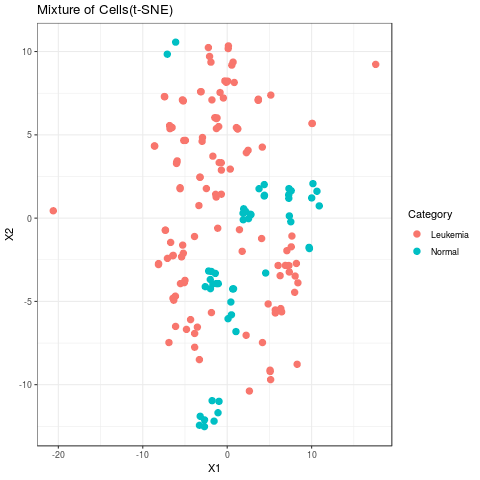
\includegraphics{img/mixtSNE.png}}{}
	\makeatother 
	\caption{{T-SNE indicates poor separability in cell mixture.}}
	\label{f-c2b15a1bach9}
\end{figure*}
\egroup
\bgroup
\fixFloatSize{img/TtSNE.png}
\begin{figure*}[!htbp]
	\centering \makeatletter\IfFileExists{img/TtSNE.png}{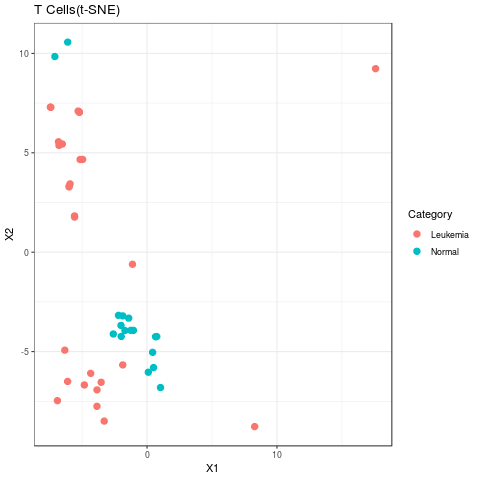
\includegraphics{img/TtSNE.png}}{}
	\makeatother 
	\caption{{T-SNE indicates relatively better separability in T cells.}}
	\label{f-c2b15a1baci9}
\end{figure*}
\egroup
\bgroup
\fixFloatSize{img/BtSNE.png}
\begin{figure*}[!htbp]
	\centering \makeatletter\IfFileExists{img/BtSNE.png}{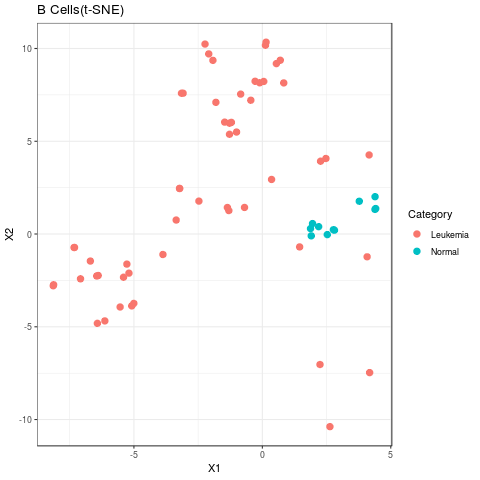
\includegraphics{img/BtSNE.png}}{}
	\makeatother 
	\caption{{T-SNE indicates almost perfect separability in B cells.}}
	\label{f-c2b15a1bacj9}
\end{figure*}
\egroup
\bgroup
    
In spite of data not being separable and cluster-able satisfyingly while looking as a whole, no portion of it was eliminated and the data analysis was done even once with the whole data, supporting the results acquired in subgroups analyses.

\section{Differential Expression Analysis}
This article has employed \cite{Cramer-Morales1293} data set and Limma tools (\cite{10.1093/nar/gkv007}.) The data set primarily consists of 170 samples having their expressions measured by 32321 probes and classified in two categories, having self-explanatory labels, "Normal" and "Leukemia." These samples were first examined in three prospectives, respectively independent of the cell source, cells of type T, cells of type B(Table~\ref{tw-791fc4df10f0}.)

After having the data in this format, a basic visualization was employed to form an intuition about the comparability of the data. The data needed no normalization (figure1.) However, the heatmap and its interensic hierarchical clustering failed to assure the validity of the data.


\begin{table*}[!htbp]
\caption{{The samples were studied dependant and independant of their source.} }
\label{tw-791fc4df10f0}
\def\arraystretch{1}
\ignorespaces 
\centering 
\begin{tabulary}{\linewidth}{p{\dimexpr.2452\linewidth-2\tabcolsep}p{\dimexpr.41480000000000004\linewidth-2\tabcolsep}p{\dimexpr.34\linewidth-2\tabcolsep}}
\tbltoprule Source Dependancy & Normal Sources & Leukemia Sources\\
\tblmidrule 
Independent &
  B Cells, CD34+HSPC, Granulocytes, Monocytes, T Cells &
  AML Cell Line, AML Patient, B ALL Cell Line, B ALL Patient, T ALL Cell Line, T ALL Patient\\
T cells &
  T Cells &
  T ALL Cell Line, T ALL Patient\\
B cells &
  B Cells &
  B ALL Cell Line, B ALL Patient\\
 &
   &
  \\
\tblbottomrule 
\end{tabulary}\par 
\end{table*}
extract some genes with significantly different expression levels in normal versus affected cells.


    
\section{Gene Set Enrichment Analysis}
As the gene sets extracted, they were passed to EnrichR to find possible causes and cures for AML. The GSEA results were truncated not to be represent ideas elusive to naked eyes. So only results with adjusted p-value less than .05 were selected. Moreover, at most 5 top cases extracted from each database were kept and the rest were eliminated. The results were sorted by combined score before the elimination process. The databases that were exploited for each purpose are listed in Table~\ref{tw-de478ae31cc6} . \ref{appendix-title-1f696b9ef905} would explain the reason of each database choice.


\begin{table*}[!htbp]
\caption{{Databases in Use for GSEA} }
\label{tw-de478ae31cd6}
\def\arraystretch{1}
\ignorespaces 
\centering 
\begin{tabulary}{\linewidth}{p{\dimexpr.2732\linewidth-2\tabcolsep}p{\dimexpr.7267999999999999\linewidth-2\tabcolsep}}
\tbltoprule Analysis & Databases\\
\tblmidrule 
Transcription Factors &
  TRANSFAC and JASPAR PWMs, miRTarBase 2017\\
Pathways &
  KEGG2019 Human, NCI-Nature 2016, Reactome 2016\\
Gene Ontology &
  GO Biological Process 2018, GO Molecular Function 2018, GO Cellular Component 2018\\
Drugs &
  ARCHS4 IDG Coexp\\
\tblbottomrule 
\end{tabulary}\par 
\end{table*}
The comprehensive genes outputed by GSEA can be viewed in\ref{appendix-title-fe590e9f8eaf}. Amongth the extracted genes, pathways, etc, some were more attractive and listed here with some details. The headers are represented in the format of ([Source\_Change], Name, Adjusted P-value, Z-score, Combined Score, database.)

\cleardoublepage

\subsection{Transcription Factors (TFs)}This section has been widely influenced by proteinatlas and  KEGG.

\subsubsection{ETV4}Transcription regulator, e.g is unfavorable to liver cancer while favorable to thyroid cancer.

\subsubsection{E2F4}Transcription facator, significant role in cell cycle regulation. 

\subsubsection{E2F1}Transcription factor of the E2F TF family.

\subsubsection{NRF1}Nuclear respiratory factor 1, TF regulating key metabolic genes.

\subsubsection{NFIC}TF in cells and replication factor for adenovirus. 

\subsubsection{NFYA}TF associated with a subunit of a high specified and affined DNA binding complex.

\subsubsection{POU2F1}Of the same group of oct4 i.e octamer transcription factors.

\subsection{Pathways (PWs)}

\subsubsection{Glycosaminoglycan degradation}
Glycosaminoglycans are polar molecules found in extracellular matrix and interact with growth factors (\cite{doi:10.3109/10409239509083490}).

\subsubsection{Glycosphingolipid biosynthesis}
Glycosphingolipids form a major part of lipid rafts in cell membrane, in which some receptors lay (\cite{Glycosphingolipids}).

\subsubsection{RIG-I-like receptor signaling pathway}
RIG-I-like receptors have accepted the role of pathogen sensing of RNA viruses (\cite{Loo2011}).

\subsubsection{Autoimmune thyroid disease}
A disease in which thyroid cells are defected and secrete antigens consequently, attracting B and T cells toward themselves, therefore, driven to necrosis/apoptosis. (\cite{KEGG ATD})

\subsubsection{Graft-versus-host disease}
Allogeneic hematopoietic transplantations causes some disorders invoking donor cells against the host ones. (\cite{Ferrara2009}, \cite{GvHD})

\subsubsection{Endosomal/Vacuolar pathway}
Antigenic peptides are generated and cross presented, resulting in loaded MHC-I cells through this pathway. (\cite{Reactome E/V P})

\subsubsection{Interferon alpha/beta signaling}
The Interferon alpha/beta signaling pathway results in some IFN-stimulated and -induced gene expressions and site bindings.
(\cite{Reactome INFA/B sig})

\subsubsection{Antigen Presentation: Folding, assembly and peptide loading of class I MHC}
Antigen peptides are loaded to MHC I molecules and cytotoxic T cells are invoked by them. This pathway deals with MHC since Folding in Golgi up to the peptide loading of it.

\subsubsection{Immune System}
Self explanatory.

\subsubsection{Interferon gamma signaling}
Interferon Gamma Receptors induce phosphorylation upon binding to IFNG and consequently activate genes containing gamma-interferon activation sequence (GAS) in their promoter along this pathway. (\cite{Reactome INFG sig})

\subsubsection{DNA replication}
Self explanatory.

\subsubsection{Homologous recombination}
A pathway in which double strand breaks are fixed using the homologous DNA sequence, which is a necessary error correction mechanism for the DNA replication. (\cite{Reacombination})

\subsubsection{Oocyte meiosis}
The process of forming mature female gametocyte.

\subsubsection{Fanconi anemia pathway}
A pathway in which some replication barriers are removed. (\cite{Rodríguez2017})

\subsubsection{E2F transcription factor network}
E2F factors are of the most important S-phase entry in the cell cycle, although their roles are not limited to the aforementioned one. (\cite{Dimova2005})

\subsubsection{PLK1 signaling events}
Yet another pathway to ensure the mitosis is done correctly. (\cite{Lera2016})

\subsubsection{FOXM1 transcription factor network}
FOXM1 TFs have been found to be essential for mitotic progression and some gene encodings as well. (\cite{Wang2005})

\subsubsection{Aurora B signaling}
Aurora B is assigned the duty of chromosome separation during cell divisions by the evolution. (\cite{Krenn2015})
It is alleged that some aneuploidies are the consecuence of its malfunctioning.

\subsubsection{ATR signaling pathway}
DNA damage response is a mechanism in cell that maintains DNA integrity. This mechanism is mainly regulated by ATR signaling pathway. (\cite{Nam2011})

\subsubsection{Cell Cycle}
A process including but not limited to DNA replication and organelle division in order to form daughter cells.

\subsubsection{M Phase}
A phase of cell cycle in which nuclear and cytoplasm are divided to form two daughter cells.

\subsubsection{Cell Cycle Checkpoints}
In order to have the cell cycle under control, evolution has defined some checkpoints between each two consecutive phases of cell cycle to ensure whether it is necessary to continue the cycle.

\subsubsection{G2/M Checkpoints}
Before entering mitosis phase, this checkpoint would check the DNA replication fidelity. (\cite{Stark2004}) 

\subsubsection{Th17 cell differentiation}
Th17 cells are a subset of CD4+ T cells. (\cite{KEGG ThCD})

\subsubsection{Allograft rejection}
The process of recognizing donor cells as intruders and attacking them by T cells. (\cite{Martinu2011})

\subsubsection{TNF receptor signaling pathway}
Regulation of cell proliferation , differentiation, and apoptosis are processes in which TNF involves in. (\cite{TNFR P sig})

\subsubsection{TRAIL signaling pathway}
TRIAL is a death ligand which binds to death receptors and causes apoptosis. Metastasis suppression is of its main roles. (\cite{Thorburn2007})

\subsubsection{IL12-mediated signaling events}
IL12 is a protein defending cell against intracellular viral infections attracting imune system against the corrupted cell. (\cite{Liu2005})

\subsubsection{Downstream signaling in naive CD8+ T cells}
%(TODO )

\subsubsection{Cytokine Signaling in Immune system}
"Cytokines are small proteins that regulate and mediate immunity, inflammation, and hematopoiesis. They are secreted in response to immune stimuli, and usually act briefly, locally, at very low concentrations." (\cite{Reactome C sig in IS})

\subsubsection{p73 transcription factor network}
p73 is a TF with low frequency of mutation in cancer despite of overlapping gene targets with p53 (\cite{Yu2006})

\subsubsection{Mitotic Prometaphase}
A phase of mitosis in which the nuclear membrane breaks apart.

\subsubsection{Resolution of Sister Chromatid Cohesion}
Eliminating cohesin complexes from chromosomes having them still connected at centromeres (\cite{Reactome RSCC})

\subsubsection{Intestinal immune network for IgA production}
A mechanism of generating and differentiating noninflammatory immunoglobulin A originated from mucosal B cells. (\cite{KEGG  IINIP})

\subsubsection{TNF signaling pathway}
TNFs play wide range of roles varying from apoptosis to survival reactions. (\cite{KEGG TNF sig})

\subsubsection{Asthma}
A pathway in which allergens invoke T cells against themselves causing inflammation. (\cite{KEGG Athma})

\subsubsection{Immunoregulatory interactions between a Lymphoid and a non-Lymphoid cell}
There are some receptors and surface attaching molecules which adjust the response of lymphoid cells to the environmental condition. (\cite{Reactome IIbLnL})

\subsubsection{Adaptive Immune System}
A major strategy of the immune system is to produce and devote a specific kind of cells to each pathogen. This is the responsibility of Adaptive Immune System.

\subsubsection{CD22 mediated BCR regulation}
Out of control BCR expression, which causes autoimmune disease, is avoided a set of mechanisms including CD22 receptors signaling. (\cite{Reactome CD22 BCR R})

\subsubsection{TNF receptor superfamily (TNFSF) members mediating non-canonical NF-kB pathway}
%(TODO )

\subsubsection{Human T-cell leukemia virus 1 infection}
A retroviral infection mostly nonlethal and even asymptomatic. (\cite{TCLv1})

\subsubsection{Regulation of retinoblastoma protein}
Of the main G0/G1 and G1/S regulators, Rb proteins can be made. They regulates target genes of E2F TFs. (\cite{Hume2009})

\subsubsection{Mitotic G1-G1/S phases}
Respectively growth focused and transition states in which cell's commitment to the proliferation is ensured. (\cite{Bertoli2013})
\newline \newline
It can be obviously observed that the listed pathways are mainly concerning cell cycle and immune system. It can be guessed that cell cycle regulation errors are the causes of AML, while immune system deficiencies are the consequences of the cancer. The former is widely studied in \cite{Saito2010}, \cite{Stiehl940}, \cite{BANKER1998221}, \cite{Schnerch2012}, and a handful of other articles. This article would follow the later to compile pieces of information about immune system deficiencies and AML relation.

\subsection{Gene Ontology}
Table %(TODO: )
up to Table %(TODO: )
would cover extracted Gene Ontologies which are in simple English and, therefore, intelligible using only high school biology knowledge.
Skimming through tables entries, it was observed that highly scored ontologies are strongly linked to cell cycle regulation and fidelity mechanisms, and cellular components. While low scored ontologies, which are usually observed among genes which have been expressed less in AML affected cells, seems related to immune system regulation mechanisms and actions. Exploiting existing knowledge about AML, it could be inferred that due to failure of immune cells to differentiate and become mature, they lack the ability to accomplish their normal responsibility. Hence, the idea of immune deficiencies be side effects of AML is supported.

\subsection{Consensus}
As retroviral infections are not reported as significant causes of AML, it is not a strong suggestion to regard immune system weakness a major cause of AML. However, \cite{Ramadan2012} has indicated that autoimmune deficiencies can surge the risk of AML and supported this idea with a number of statistical tests. These tests approve the claim in some cases while stay wordless against others. Moreover, the immune system can be considered as a major therapy fails in AML. Bone marrow stem cell transplant is among the most well known therapies for AML while as indicated by \cite{Horowitz555} it is suppressed by body immune system and donor cells are identified as intruders by the immune system. Previously reported pathways in this article has pointed this out. \cite{Lamble2018} suggests immunotherapy methods to bypass the aforementioned problem.

\subsection{Drugs}
Usually cancer drugs target cell cycle phases to regulate the cell cycle, hoping to outperform mutational adaption of cancer cells (\cite{Shapiro1999}, \cite{Bai2017}. A list of less studied drugs can be found in (TODO appx)
, but due to the god damn deadline, any investigation about docking capability and other related drug assessments are ignored.

\subsection{Future Works}
During the study, two main challenges were faced. The first one was the absence of a clustering and separability metric with a reasonable biological interpretation which had left the researcher unsure whether to ignore some samples for the sake of accuracy. A workaround was to define a metric based on the variance in each cluster using only its data label. The second challenge was the absence of an automated tool to relate the enrichment analysis results to each other. A proposed idea which is supported by intuition but suffering major drawbacks is to feed the enrichment process again using the extracted TFs. This idea was tested and provided weak statistical results.

\section*{Acknowledgments} Special thanks to the teaching team and author's patient classmates, who were a great source of inspiration and knowledge.

\appendix

\section{GSEA Database Selection}\label{appendix-title-1f696b9ef905}
TRANSFAC and JASPAR PWMs, and miRTarBase 2017 were chosen for TF enrichment because they were curated and validated experimentally. KEGG and Reactome was selected for the same reason, however due to its vast resources and manually curated essence, NCI-Nature was used as well.
Once again, being manually curated, was an advantage of GO against Jensen group. ARCHS4 IDG Coexp was interesting for the research because of the article's approach of digging into less studied areas has been satisfied by it. In fact, ARCHS4 IDG Coexp covers numerous under-studied drugs.



\section{GSEA Full Selected Genes}\label{appendix-title-fe590e9f8eaf}
\begin{table*}[!htbp]
	\caption{{TF Analysis of genes under-expressed in AML (cell mixture), TRANSFAC and JASPAR PWMs} }
	\label{tw-de478ae31ce6}
	\def\arraystretch{1}
	\ignorespaces 
	\centering 
	\begin{tabulary}{\linewidth}{p{\dimexpr.65\linewidth-2\tabcolsep}p{\dimexpr.15\linewidth-2\tabcolsep}p{\dimexpr.1\linewidth-2\tabcolsep}p{\dimexpr.1\linewidth-2\tabcolsep}}
		\tbltoprule Name & Adj. P-value & Z-score & Combined Score\\
		\tblmidrule 
ETV4 (human) & 0.043 & -1.74 & 15.24  \\
		\tblbottomrule
	\end{tabulary}\par 
\end{table*}
\begin{table*}[!htbp]
	\caption{{TF Analysis of genes over-expressed in AML (cell mixture), TRANSFAC and JASPAR PWMs} }
	\label{tw-de478ae31cf6}
	\def\arraystretch{1}
	\ignorespaces 
	\centering 
	\begin{tabulary}{\linewidth}{p{\dimexpr.65\linewidth-2\tabcolsep}p{\dimexpr.15\linewidth-2\tabcolsep}p{\dimexpr.1\linewidth-2\tabcolsep}p{\dimexpr.1\linewidth-2\tabcolsep}}
		\tbltoprule Name & Adj. P-value & Z-score & Combined Score\\
		\tblmidrule 
E2F4 (human) & 6.248e-9 & -1.97 & 48.40 \\
E2F1 (human) & 0.00002605 & -1.55 & 23.43 \\
NRF1 (human) & 0.0001446 & -1.71 & 22.44 \\
NFIC (human) & 0.001465 & -1.69 & 18.00 \\
NFYA (human) & 0.002248 & -1.60 & 16.03 \\
		\tblbottomrule
	\end{tabulary}\par 
\end{table*}
\begin{table*}[!htbp]
	\caption{{TF Analysis of genes over-expressed in AML (cell mixture), miRTarBase 2017} }
	\label{tw-de478ae31cg6}
	\def\arraystretch{1}
	\ignorespaces 
	\centering 
	\begin{tabulary}{\linewidth}{p{\dimexpr.65\linewidth-2\tabcolsep}p{\dimexpr.15\linewidth-2\tabcolsep}p{\dimexpr.1\linewidth-2\tabcolsep}p{\dimexpr.1\linewidth-2\tabcolsep}}
		\tbltoprule Name & Adj. P-value & Z-score & Combined Score\\
		\tblmidrule
hsa-miR-193b-3p & 8.760050e-64 & -6.364176 & 973.9777 \\
hsa-miR-192-5p & 2.501043e-31 & -6.765765 & 522.3863 \\
hsa-miR-215-5p & 2.718386e-34 & -5.184328 & 437.7653 \\
hsa-miR-34a-5p & 9.159129e-21 & -5.117180 & 269.1568 \\
hsa-miR-92a-3p & 1.886866e-08 & -9.381637 & 223.6528 \\
		\tblbottomrule
	\end{tabulary}\par 
\end{table*}
\begin{table*}[!htbp]
	\caption{{TF Analysis of genes over-expressed in AML (T Cells), TRANSFAC and JASPAR PWMs} }
	\label{tw-de478ae31ch6}
	\def\arraystretch{1}
	\ignorespaces 
	\centering 
	\begin{tabulary}{\linewidth}{p{\dimexpr.65\linewidth-2\tabcolsep}p{\dimexpr.15\linewidth-2\tabcolsep}p{\dimexpr.1\linewidth-2\tabcolsep}p{\dimexpr.1\linewidth-2\tabcolsep}}
		\tbltoprule Name & Adj. P-value & Z-score & Combined Score\\
		\tblmidrule
E2F4 (human) & 0.006586 & -1.95 & 18.87 \\
E2F1 (human) & 0.002198 & -1.57 & 18.41 \\
		\tblbottomrule
	\end{tabulary}\par 
\end{table*}
\begin{table*}[!htbp]
	\caption{{TF Analysis of genes over-expressed in AML (T Cells), miRTarBase 2017} }
	\label{tw-de478ae31ci6}
	\def\arraystretch{1}
	\ignorespaces 
	\centering 
	\begin{tabulary}{\linewidth}{p{\dimexpr.65\linewidth-2\tabcolsep}p{\dimexpr.15\linewidth-2\tabcolsep}p{\dimexpr.1\linewidth-2\tabcolsep}p{\dimexpr.1\linewidth-2\tabcolsep}}
		\tbltoprule Name & Adj. P-value & Z-score & Combined Score\\
		\tblmidrule
hsa-miR-193b-3p & 1.574e-35 & -6.36 & 558.85 \\
hsa-miR-192-5p & 4.991e-29 & -6.77 & 485.40 \\
hsa-miR-215-5p & 6.399e-30 & -5.18 & 384.69 \\
hsa-miR-34a-5p & 1.639e-7 & -5.12 & 112.13 \\
hsa-let-7b-5p & 0.008490 & -7.90 & 85.63 \\
		\tblbottomrule
	\end{tabulary}\par 
\end{table*}
\begin{table*}[!htbp]
	\caption{{TF Analysis of genes under-expressed in AML (B Cells), TRANSFAC and JASPAR PWMs} }
	\label{tw-de478ae31cj6}
	\def\arraystretch{1}
	\ignorespaces 
	\centering 
	\begin{tabulary}{\linewidth}{p{\dimexpr.65\linewidth-2\tabcolsep}p{\dimexpr.15\linewidth-2\tabcolsep}p{\dimexpr.1\linewidth-2\tabcolsep}p{\dimexpr.1\linewidth-2\tabcolsep}}
		\tbltoprule Name & Adj. P-value & Z-score & Combined Score\\
		\tblmidrule
POU2F1 (human) & 0.03246 & -1.74 & 15.68 \\
		\tblbottomrule
	\end{tabulary}\par 
\end{table*}
\begin{table*}[!htbp]
	\caption{{TF Analysis of genes over-expressed in AML (B Cells), TRANSFAC and JASPAR PWMs} }
	\label{tw-de478ae31ck6}
	\def\arraystretch{1}
	\ignorespaces 
	\centering 
	\begin{tabulary}{\linewidth}{p{\dimexpr.65\linewidth-2\tabcolsep}p{\dimexpr.15\linewidth-2\tabcolsep}p{\dimexpr.1\linewidth-2\tabcolsep}p{\dimexpr.1\linewidth-2\tabcolsep}}
		\tbltoprule Name & Adj. P-value & Z-score & Combined Score\\
		\tblmidrule
E2F4 (human) & 3.861e-8 & -1.97 & 44.58 \\
E2F1 (human) & 0.005012 & -1.55 & 15.12 \\
NRF1 (human) & 0.01787 & -1.71 & 14.02 \\
		\tblbottomrule
	\end{tabulary}\par 
\end{table*}
\begin{table*}[!htbp]
	\caption{{TF Analysis of genes over-expressed in AML (B Cells), miRTarBase 2017} }
	\label{tw-de478ae31cl6}
	\def\arraystretch{1}
	\ignorespaces 
	\centering 
	\begin{tabulary}{\linewidth}{p{\dimexpr.65\linewidth-2\tabcolsep}p{\dimexpr.15\linewidth-2\tabcolsep}p{\dimexpr.1\linewidth-2\tabcolsep}p{\dimexpr.1\linewidth-2\tabcolsep}}
		\tbltoprule Name & Adj. P-value & Z-score & Combined Score\\
		\tblmidrule
hsa-miR-193b-3p & 1.275e-39 & -6.36 & 618.57 \\
hsa-miR-192-5p & 4.036e-18 & -6.77 & 315.22 \\
hsa-miR-215-5p & 2.494e-19 & -5.18 & 258.08 \\
hsa-miR-34a-5p & 5.211e-14 & -5.12 & 188.50 \\
hsa-let-7b-5p & 0.00006949 & -7.90 & 121.79 \\
		\tblbottomrule
	\end{tabulary}\par 
\end{table*}
\begin{table*}[!htbp]
	\caption{{PW Analysis of genes under-expressed in AML (cell mixture), KEGG2019 Human} }
	\label{tw-de478ae31cm6}
	\def\arraystretch{1}
	\ignorespaces 
	\centering 
	\begin{tabulary}{\linewidth}{p{\dimexpr.65\linewidth-2\tabcolsep}p{\dimexpr.15\linewidth-2\tabcolsep}p{\dimexpr.1\linewidth-2\tabcolsep}p{\dimexpr.1\linewidth-2\tabcolsep}}
		\tbltoprule Name & Adj. P-value & Z-score & Combined Score\\
		\tblmidrule
Glycosaminoglycan degradation & 0.02246 & -613.78 & 3210.85 \\
Glycosphingolipid biosynthesis & 0.4322 & -900.86 & 1321.91 \\
RIG-I-like receptor signaling pathway & 0.004278 & -97.67 & 704.97 \\
Autoimmune thyroid disease & 0.002948 & -78.88 & 653.40 \\
Graft-versus-host disease & 0.001461 & -68.48 & 636.28 \\
		\tblbottomrule
	\end{tabulary}\par 
\end{table*}
\begin{table*}[!htbp]
	\caption{{PW Analysis of genes under-expressed in AML (cell mixture), Reactome 2016} }
	\label{tw-de478ae31cn6}
	\def\arraystretch{1}
	\ignorespaces 
	\centering 
	\begin{tabulary}{\linewidth}{p{\dimexpr.65\linewidth-2\tabcolsep}p{\dimexpr.15\linewidth-2\tabcolsep}p{\dimexpr.1\linewidth-2\tabcolsep}p{\dimexpr.1\linewidth-2\tabcolsep}}
		\tbltoprule Name & Adj. P-value & Z-score & Combined Score\\
		\tblmidrule
Endosomal/Vacuolar pathway\_Homo sapiens\_R-HSA-1236977 & 0.000001320 & -1.98 & 37.94 \\
Interferon alpha/beta signaling\_Homo sapiens\_R-HSA-909733 & 0.00001904 & -1.86 & 29.37 \\
Antigen Presentation: Folding, assembly and peptide loading of class I MHC\_Homo sapiens\_R-HSA-983170 & 0.00002778 & -1.93 & 28.99 \\
Immune System\_Homo sapiens\_R-HSA-168256 & 0.0001276 & -2.20 & 28.61 \\
Interferon gamma signaling\_Homo sapiens\_R-HSA-877300 & 0.00008257 & -1.76 & 24.06 \\
		\tblbottomrule
	\end{tabulary}\par 
\end{table*}
\begin{table*}[!htbp]
	\caption{{PW Analysis of genes over-expressed in AML (cell mixture), KEGG2019 Human} }
	\label{tw-de478ae31co6}
	\def\arraystretch{1}
	\ignorespaces 
	\centering 
	\begin{tabulary}{\linewidth}{p{\dimexpr.65\linewidth-2\tabcolsep}p{\dimexpr.15\linewidth-2\tabcolsep}p{\dimexpr.1\linewidth-2\tabcolsep}p{\dimexpr.1\linewidth-2\tabcolsep}}
		\tbltoprule Name & Adj. P-value & Z-score & Combined Score\\
		\tblmidrule
DNA replication	6.096e-17 & -49.69 & 1855.26 &  \\
Homologous recombination & 5.327e-9 & -49.65 & 1100.04 \\
Oocyte meiosis & 1.312e-10 & -26.82 & 704.47 \\
Fanconi anemia pathway & 0.000001224 & -41.92 & 687.64 \\
Small cell lung cancer & 0.0006399 & -63.94 & 602.21 \\
		\tblbottomrule
	\end{tabulary}\par 
\end{table*}
\begin{table*}[!htbp]
	\caption{{PW Analysis of genes over-expressed in AML (cell mixture), NCI-Nature} }
	\label{tw-de478ae31cp6}
	\def\arraystretch{1}
	\ignorespaces 
	\centering 
	\begin{tabulary}{\linewidth}{p{\dimexpr.65\linewidth-2\tabcolsep}p{\dimexpr.15\linewidth-2\tabcolsep}p{\dimexpr.1\linewidth-2\tabcolsep}p{\dimexpr.1\linewidth-2\tabcolsep}}
		\tbltoprule Name & Adj. P-value & Z-score & Combined Score\\
		\tblmidrule
E2F transcription factor network\_Homo sapiens\_bb4d0fd3-6191-11e5-8ac5-06603eb7f303 & 1.616e-20 & -1.73 & 85.49 \\
PLK1 signaling events\_Homo sapiens\_e5e87977-6194-11e5-8ac5-06603eb7f303 & 1.127e-20 & -1.66 & 83.87 \\
FOXM1 transcription factor network\_Homo sapiens\_c51cda49-6192-11e5-8ac5-06603eb7f303 & 2.769e-16 & -1.51 & 58.67 \\
Aurora B signaling\_Homo sapiens\_304a75af-618c-11e5-8ac5-06603eb7f303 & 5.779e-18 & -1.26 & 54.28 \\
ATR signaling pathway\_Homo sapiens\_8991cbac-618b-11e5-8ac5-06603eb7f303 & 4.751e-15 & -1.18 & 42.36 \\
		\tblbottomrule
	\end{tabulary}\par 
\end{table*}
\begin{table*}[!htbp]
	\caption{{PW Analysis of genes over-expressed in AML (cell mixture), Reactome 2016} }
	\label{tw-de478ae31cq6}
	\def\arraystretch{1}
	\ignorespaces 
	\centering 
	\begin{tabulary}{\linewidth}{p{\dimexpr.65\linewidth-2\tabcolsep}p{\dimexpr.15\linewidth-2\tabcolsep}p{\dimexpr.1\linewidth-2\tabcolsep}p{\dimexpr.1\linewidth-2\tabcolsep}}
		\tbltoprule Name & Adj. P-value & Z-score & Combined Score\\
		\tblmidrule
Cell Cycle\_Homo sapiens\_R-HSA-1640170 & 1.426e-117 & -2.46 & 677.98 \\
Cell Cycle, Mitotic\_Homo sapiens\_R-HSA-69278 & 1.227e-106 & -2.47 & 616.03 \\
M Phase\_Homo sapiens\_R-HSA-68886 & 2.552e-50 & -2.43 & 290.68 \\
Cell Cycle Checkpoints\_Homo sapiens\_R-HSA-69620 & 6.168e-44 & -2.34 & 244.94 \\
G2/M Checkpoints\_Homo sapiens\_R-HSA-69481 & 2.432e-40 & -2.32 & 222.45 \\
		\tblbottomrule
	\end{tabulary}\par 
\end{table*}
\begin{table*}[!htbp]
	\caption{{PW Analysis of genes under-expressed in AML (T Cells), KEGG2019 Human} }
	\label{tw-de478ae31cr6}
	\def\arraystretch{1}
	\ignorespaces 
	\centering 
	\begin{tabulary}{\linewidth}{p{\dimexpr.65\linewidth-2\tabcolsep}p{\dimexpr.15\linewidth-2\tabcolsep}p{\dimexpr.1\linewidth-2\tabcolsep}p{\dimexpr.1\linewidth-2\tabcolsep}}
		\tbltoprule Name & Adj. P-value & Z-score & Combined Score\\
		\tblmidrule
Glycosaminoglycan degradation & 0.1424 & -585.89 & 2091.24 \\
Autoimmune thyroid disease & 0.00003361 & -80.82 & 1151.46 \\
Th17 cell differentiation & 0.00002734 & -69.21 & 1041.32 \\
Graft-versus-host disease & 0.00004041 & -68.48 & 923.26 \\
Allograft rejection & 0.00003361 & -54.70 & 767.09 \\
		\tblbottomrule
	\end{tabulary}\par 
\end{table*}
\begin{table*}[!htbp]
	\caption{{PW Analysis of genes under-expressed in AML (T Cells), NCI-Nature} }
	\label{tw-de478ae31cs6}
	\def\arraystretch{1}
	\ignorespaces 
	\centering 
	\begin{tabulary}{\linewidth}{p{\dimexpr.65\linewidth-2\tabcolsep}p{\dimexpr.15\linewidth-2\tabcolsep}p{\dimexpr.1\linewidth-2\tabcolsep}p{\dimexpr.1\linewidth-2\tabcolsep}}
		\tbltoprule Name & Adj. P-value & Z-score & Combined Score\\
		\tblmidrule
TNF receptor signaling pathway\_Homo sapiens\_316be05e-6196-11e5-8ac5-06603eb7f303 & 0.0001737 & -1.53 & 19.39 \\
TRAIL signaling pathway\_Homo sapiens\_3a79fddf-6196-11e5-8ac5-06603eb7f303 & 0.0001737 & -1.41 & 18.49 \\
IL12-mediated signaling events\_Homo sapiens\_7acdea19-6193-11e5-8ac5-06603eb7f303 & 0.0008804 & -1.54 & 16.39 \\
Downstream signaling in naive CD8+ T cells\_Homo sapiens\_92180cef-6191-11e5-8ac5-06603eb7f303 & 0.0009973 & -1.43 & 14.59 \\
IL2-mediated signaling events\_Homo sapiens\_a2a1883c-6193-11e5-8ac5-06603eb7f303 & 0.002484 & -1.55 & 14.07 \\
		\tblbottomrule
	\end{tabulary}\par 
\end{table*}
\begin{table*}[!htbp]
	\caption{{PW Analysis of genes under-expressed in AML (T Cells), Reactome 2016} }
	\label{tw-de478ae31ct6}
	\def\arraystretch{1}
	\ignorespaces 
	\centering 
	\begin{tabulary}{\linewidth}{p{\dimexpr.65\linewidth-2\tabcolsep}p{\dimexpr.15\linewidth-2\tabcolsep}p{\dimexpr.1\linewidth-2\tabcolsep}p{\dimexpr.1\linewidth-2\tabcolsep}}
		\tbltoprule Name & Adj. P-value & Z-score & Combined Score\\
		\tblmidrule
Immune System\_Homo sapiens\_R-HSA-168256 & 0.00001975 & -2.23 & 37.84 \\
Cytokine Signaling in Immune system\_Homo sapiens\_R-HSA-1280215 & 0.00003972 & -2.40 & 37.28 \\
Endosomal/Vacuolar pathway\_Homo sapiens\_R-HSA-1236977 & 0.00004649 & -1.90 & 28.15 \\
Interferon alpha/beta signaling\_Homo sapiens\_R-HSA-909733 & 0.00004649 & -1.84 & 27.00 \\
Interferon gamma signaling\_Homo sapiens\_R-HSA-877300 & 0.00006090 & -1.75 & 24.90 \\
		\tblbottomrule
	\end{tabulary}\par 
\end{table*}
\begin{table*}[!htbp]
	\caption{{PW Analysis of genes over-expressed in AML (T Cells), KEGG2019 Human} }
	\label{tw-de478ae31cu6}
	\def\arraystretch{1}
	\ignorespaces 
	\centering 
	\begin{tabulary}{\linewidth}{p{\dimexpr.65\linewidth-2\tabcolsep}p{\dimexpr.15\linewidth-2\tabcolsep}p{\dimexpr.1\linewidth-2\tabcolsep}p{\dimexpr.1\linewidth-2\tabcolsep}}
		\tbltoprule Name & Adj. P-value & Z-score & Combined Score\\
		\tblmidrule
Glyoxylate and dicarboxylate metabolism & 0.5917 & -701.48 & 867.99 \\
Glycosaminoglycan biosynthesis & 0.3410 & -406.31 & 856.52 \\
Homologous recombination & 0.00001242 & -50.16 & 744.50 \\
Small cell lung cancer & 0.001191 & -67.62 & 628.70 \\
DNA replication & 0.00006099 & -49.02 & 624.51 \\
		\tblbottomrule
	\end{tabulary}\par 
\end{table*}
\begin{table*}[!htbp]
	\caption{{PW Analysis of genes over-expressed in AML (T Cells), NCI-Nature} }
	\label{tw-de478ae31cv6}
	\def\arraystretch{1}
	\ignorespaces 
	\centering 
	\begin{tabulary}{\linewidth}{p{\dimexpr.65\linewidth-2\tabcolsep}p{\dimexpr.15\linewidth-2\tabcolsep}p{\dimexpr.1\linewidth-2\tabcolsep}p{\dimexpr.1\linewidth-2\tabcolsep}}
		\tbltoprule Name & Adj. P-value & Z-score & Combined Score\\
		\tblmidrule
PLK1 signaling events\_Homo sapiens\_e5e87977-6194-11e5-8ac5-06603eb7f303 & 1.853e-13 & -1.66 & 55.78 \\
FOXM1 transcription factor network\_Homo sapiens\_c51cda49-6192-11e5-8ac5-06603eb7f303 & 1.887e-11 & -1.65 & 46.63 \\
E2F transcription factor network\_Homo sapiens\_bb4d0fd3-6191-11e5-8ac5-06603eb7f303 & 3.319e-11 & -1.68 & 45.91 \\
p73 transcription factor network\_Homo sapiens\_a88c505e-6194-11e5-8ac5-06603eb7f303 & 8.821e-10 & -1.38 & 32.22 \\
ATR signaling pathway\_Homo sapiens\_8991cbac-618b-11e5-8ac5-06603eb7f303 & 1.914e-10 & -1.24 & 31.11 \\
		\tblbottomrule
	\end{tabulary}\par 
\end{table*}
\begin{table*}[!htbp]
	\caption{{PW Analysis of genes over-expressed in AML (T Cells), Reactome 2016} }
	\label{tw-de478ae31cw6}
	\def\arraystretch{1}
	\ignorespaces 
	\centering 
	\begin{tabulary}{\linewidth}{p{\dimexpr.65\linewidth-2\tabcolsep}p{\dimexpr.15\linewidth-2\tabcolsep}p{\dimexpr.1\linewidth-2\tabcolsep}p{\dimexpr.1\linewidth-2\tabcolsep}}
		\tbltoprule Name & Adj. P-value & Z-score & Combined Score\\
		\tblmidrule
Cell Cycle\_Homo sapiens\_R-HSA-1640170 & 3.743e-54 & -2.46 & 317.68 \\
Cell Cycle, Mitotic\_Homo sapiens\_R-HSA-69278 & 5.027e-44 & -2.47 & 259.31 \\
Mitotic Prometaphase\_Homo sapiens\_R-HSA-68877 & 1.905e-22 & -2.03 & 111.73 \\
M Phase\_Homo sapiens\_R-HSA-68886 & 2.687e-18 & -2.41 & 107.58 \\
Resolution of Sister Chromatid Cohesion\_Homo sapiens\_R-HSA-2500257 & 1.644e-20 & -2.06 & 103.70 \\
Intestinal immune network for IgA production & 0.000003880 & -99.15 & 1739.13 \\
		\tblbottomrule
	\end{tabulary}\par 
\end{table*}
\begin{table*}[!htbp]
	\caption{{PW Analysis of genes under-expressed in AML (B Cells), KEGG2019 Human} }
	\label{tw-de478ae31cx6}
	\def\arraystretch{1}
	\ignorespaces 
	\centering 
	\begin{tabulary}{\linewidth}{p{\dimexpr.65\linewidth-2\tabcolsep}p{\dimexpr.15\linewidth-2\tabcolsep}p{\dimexpr.1\linewidth-2\tabcolsep}p{\dimexpr.1\linewidth-2\tabcolsep}}
		\tbltoprule Name & Adj. P-value & Z-score & Combined Score\\
		\tblmidrule
Glycosphingolipid biosynthesis & 0.8842 & -781.54 & 574.04 \\
TNF signaling pathway & 0.06974 & -74.45 & 391.55 \\
Autoimmune thyroid disease & 0.08780 & -77.59 & 383.98 \\
Asthma & 0.09760 & -81.53 & 76.60 \\
		\tblbottomrule
	\end{tabulary}\par 
\end{table*}
\begin{table*}[!htbp]
	\caption{{PW Analysis of genes under-expressed in AML (B Cells), Reactome 2016} }
	\label{tw-de478ae31cy6}
	\def\arraystretch{1}
	\ignorespaces 
	\centering 
	\begin{tabulary}{\linewidth}{p{\dimexpr.65\linewidth-2\tabcolsep}p{\dimexpr.15\linewidth-2\tabcolsep}p{\dimexpr.1\linewidth-2\tabcolsep}p{\dimexpr.1\linewidth-2\tabcolsep}}
		\tbltoprule Name & Adj. P-value & Z-score & Combined Score\\
		\tblmidrule
Immune System\_Homo sapiens\_R-HSA-168256 & 0.0003718 & -2.23 & 31.24 \\
Immunoregulatory interactions between a Lymphoid and a non-Lymphoid cell\_Homo sapiens\_R-HSA-198933 & 0.0006682 & -2.00 & 25.45 \\
Adaptive Immune System\_Homo sapiens\_R-HSA-1280218 & 0.006699 & 2.27 & 22.67 \\
CD22 mediated BCR regulation\_Homo sapiens\_R-HSA-5690714 & 0.009758 & -1.94 & 17.65 \\
TNF receptor superfamily (TNFSF) members mediating non-canonical NF-kB pathway\_Homo sapiens\_R-HSA-5676594 & 0.009595 & -1.88 & 17.61 \\
		\tblbottomrule
	\end{tabulary}\par 
\end{table*}
\begin{table*}[!htbp]
	\caption{{PW Analysis of genes over-expressed in AML (B Cells), KEGG2019 Human} }
	\label{tw-de478ae31cz6}
	\def\arraystretch{1}
	\ignorespaces 
	\centering 
	\begin{tabulary}{\linewidth}{p{\dimexpr.65\linewidth-2\tabcolsep}p{\dimexpr.15\linewidth-2\tabcolsep}p{\dimexpr.1\linewidth-2\tabcolsep}p{\dimexpr.1\linewidth-2\tabcolsep}}
		\tbltoprule Name & Adj. P-value & Z-score & Combined Score\\
		\tblmidrule
Small cell lung cancer & 0.002421 & -64.35 & 525.51 \\
DNA replication & 0.0004052 & -48.35 & 515.36 \\
Homologous recombination & 0.0005634 & -48.79 & 488.48 \\
Fanconi anemia pathway & 0.001818 & -40.98 & 355.37 \\
Human T-cell leukemia virus 1 infection & 0.00003497 & -18.10 & 242.43 \\
		\tblbottomrule
	\end{tabulary}\par 
\end{table*}
\begin{table*}[!htbp]
	\caption{{PW Analysis of genes over-expressed in AML (B Cells), NCI-Nature} }
	\label{tw-de478ae31dc6}
	\def\arraystretch{1}
	\ignorespaces 
	\centering 
	\begin{tabulary}{\linewidth}{p{\dimexpr.65\linewidth-2\tabcolsep}p{\dimexpr.15\linewidth-2\tabcolsep}p{\dimexpr.1\linewidth-2\tabcolsep}p{\dimexpr.1\linewidth-2\tabcolsep}}
		\tbltoprule Name & Adj. P-value & Z-score & Combined Score\\
		\tblmidrule
E2F transcription factor network\_Homo sapiens\_bb4d0fd3-6191-11e5-8ac5-06603eb7f303 & 6.635e-13 & -1.78 & 57.97 \\
FOXM1 transcription factor network\_Homo sapiens\_c51cda49-6192-11e5-8ac5-06603eb7f303 & 6.102e-9 & -1.65 & 37.63 \\
PLK1 signaling events\_Homo sapiens\_e5e87977-6194-11e5-8ac5-06603eb7f303 & 2.976e-7 & -1.47 & 26.78 \\
Aurora B signaling\_Homo sapiens\_304a75af-618c-11e5-8ac5-06603eb7f303 & 9.910e-8 & -1.26 & 24.67 \\
Regulation of retinoblastoma protein\_Homo sapiens\_407a3468-6195-11e5-8ac5-06603eb7f303 & 0.000003482 & -1.52 & 23.55 \\
		\tblbottomrule
	\end{tabulary}\par 
\end{table*}
\begin{table*}[!htbp]
	\caption{{PW Analysis of genes over-expressed in AML (B Cells), Reactome 2016} }
	\label{tw-de478ae31ec6}
	\def\arraystretch{1}
	\ignorespaces 
	\centering 
	\begin{tabulary}{\linewidth}{p{\dimexpr.65\linewidth-2\tabcolsep}p{\dimexpr.15\linewidth-2\tabcolsep}p{\dimexpr.1\linewidth-2\tabcolsep}p{\dimexpr.1\linewidth-2\tabcolsep}}
		\tbltoprule Name & Adj. P-value & Z-score & Combined Score\\
		\tblmidrule
Cell Cycle\_Homo sapiens\_R-HSA-1640170 & 1.430e-40 & -2.46 & 241.02 \\
Cell Cycle, Mitotic\_Homo sapiens\_R-HSA-69278 & 7.756e-36 & -2.47 & 213.08 \\
Mitotic G1-G1/S phases\_Homo sapiens\_R-HSA-453279 & 1.077e-18 & -2.11 & 98.22 \\
G1/S Transition\_Homo sapiens\_R-HSA-69206 & 2.942e-15 & -2.11 & 80.21 \\
Mitotic Prometaphase\_Homo sapiens\_R-HSA-68877 & 1.569e-15 & -2.02 & 78.71 \\
		\tblbottomrule
	\end{tabulary}\par 
\end{table*}
\begin{table*}[!htbp]
	\caption{{GO Analysis of genes under-expressed in AML (cell mixture), GO Biological Process 2018} }
	\label{tw-de478ae31fc6}
	\def\arraystretch{1}
	\ignorespaces 
	\centering 
	\begin{tabulary}{\linewidth}{p{\dimexpr.65\linewidth-2\tabcolsep}p{\dimexpr.15\linewidth-2\tabcolsep}p{\dimexpr.1\linewidth-2\tabcolsep}p{\dimexpr.1\linewidth-2\tabcolsep}}
		\tbltoprule Name & Adj. P-value & Z-score & Combined Score\\
		\tblmidrule
antigen processing and presentation of exogenous peptide antigen via MHC class I, TAP-independent (GO:0002480) & 0.0001851 & -2.33 & 35.76 \\
type I interferon signaling pathway (GO:0060337) & 0.0002905 & -2.32 & 30.11 \\
retrograde transport, vesicle recycling within Golgi (GO:0000301) & 0.02414 & -4.03 & 29.32 \\
regulation of necrotic cell death (GO:0010939) & 0.003712 & -2.48 & 23.91 \\
regulation of necroptotic process (GO:0060544) & 0.0002905 & -1.62 & 20.96 \\
		\tblbottomrule
	\end{tabulary}\par 
\end{table*}
\begin{table*}[!htbp]
	\caption{{GO Analysis of genes under-expressed in AML (cell mixture), GO Cellular Component 2018} }
	\label{tw-de478ae31gc6}
	\def\arraystretch{1}
	\ignorespaces 
	\centering 
	\begin{tabulary}{\linewidth}{p{\dimexpr.65\linewidth-2\tabcolsep}p{\dimexpr.15\linewidth-2\tabcolsep}p{\dimexpr.1\linewidth-2\tabcolsep}p{\dimexpr.1\linewidth-2\tabcolsep}}
		\tbltoprule Name & Adj. P-value & Z-score & Combined Score\\
		\tblmidrule
death-inducing signaling complex (GO:0031264) & 0.01076 & -3.30 & 22.26 \\
recycling endosome membrane (GO:0055038) & 0.00003093 & -1.46 & 21.80 \\
integral component of lumenal side of endoplasmic reticulum membrane (GO:0071556) & 0.001205 & -1.95 & 20.60 \\
COPII-coated ER to Golgi transport vesicle (GO:0030134) & 0.001228 & -2.06 & 19.47 \\
MHC protein complex (GO:0042611) & 0.001980 & -2.05 & 17.74 \\
		\tblbottomrule
	\end{tabulary}\par 
\end{table*}
\begin{table*}[!htbp]
	\caption{{GO Analysis of genes over-expressed in AML (cell mixture), GO Biological Process 2018} }
	\label{tw-de478ae31hc6}
	\def\arraystretch{1}
	\ignorespaces 
	\centering 
	\begin{tabulary}{\linewidth}{p{\dimexpr.65\linewidth-2\tabcolsep}p{\dimexpr.15\linewidth-2\tabcolsep}p{\dimexpr.1\linewidth-2\tabcolsep}p{\dimexpr.1\linewidth-2\tabcolsep}}
		\tbltoprule Name & Adj. P-value & Z-score & Combined Score\\
		\tblmidrule
DNA metabolic process (GO:0006259) & 1.366e-44 & -1.36 & 147.85 \\
DNA replication (GO:0006260) & 1.493e-35 & -1.56 & 135.24 \\
DNA repair (GO:0006281) & 3.977e-26 & -1.71 & 109.74 \\
mitotic cell cycle phase transition (GO:0044772) & 2.146e-32 & -1.17 & 92.67 \\
chromatin remodeling at centromere (GO:0031055) & 1.246e-15 & -2.28 & 88.85 \\
		\tblbottomrule
	\end{tabulary}\par 
\end{table*}
\begin{table*}[!htbp]
	\caption{{GO Analysis of genes over-expressed in AML (cell mixture), GO Molecular Function 2018} }
	\label{tw-de478ae31ic6}
	\def\arraystretch{1}
	\ignorespaces 
	\centering 
	\begin{tabulary}{\linewidth}{p{\dimexpr.65\linewidth-2\tabcolsep}p{\dimexpr.15\linewidth-2\tabcolsep}p{\dimexpr.1\linewidth-2\tabcolsep}p{\dimexpr.1\linewidth-2\tabcolsep}}
		\tbltoprule Name & Adj. P-value & Z-score & Combined Score\\
		\tblmidrule
DNA helicase activity (GO:0003678) & 7.421e-10 & -2.66 & 66.98 \\
ATPase activity (GO:0016887) & 4.563e-9 & -2.31 & 53.57 \\
DNA-dependent ATPase activity (GO:0008094) & 3.454e-13 & -1.53 & 51.82 \\
DNA binding (GO:0003677) & 1.223e-16 & -1.20 & 50.97 \\
3'-5' DNA helicase activity (GO:0043138) & 0.000003135 & -2.82 & 44.63 \\
		\tblbottomrule
	\end{tabulary}\par 
\end{table*}
\begin{table*}[!htbp]
	\caption{{GO Analysis of genes over-expressed in AML (cell mixture), GO Cellular Component 2018} }
	\label{tw-de478ae31jc6}
	\def\arraystretch{1}
	\ignorespaces 
	\centering 
	\begin{tabulary}{\linewidth}{p{\dimexpr.65\linewidth-2\tabcolsep}p{\dimexpr.15\linewidth-2\tabcolsep}p{\dimexpr.1\linewidth-2\tabcolsep}p{\dimexpr.1\linewidth-2\tabcolsep}}
		\tbltoprule Name & Adj. P-value & Z-score & Combined Score\\
		\tblmidrule
nuclear chromosome part (GO:0044454) & 4.133e-37 & -1.25 & 111.11 \\
chromosome, centromeric region (GO:0000775) & 5.429e-20 & -2.25 & 108.81 \\
microtubule organizing center (GO:0005815) & 1.986e-18 & -2.02 & 88.76 \\
spindle (GO:0005819) & 1.837e-29 & -1.18 & 83.06 \\
chromatin (GO:0000785) & 1.158e-19 & -1.66 & 78.42 \\
		\tblbottomrule
	\end{tabulary}\par 
\end{table*}
\begin{table*}[!htbp]
	\caption{{GO Analysis of genes under-expressed in AML (T Cells), GO Biological Process 2018} }
	\label{tw-de478ae31kc6}
	\def\arraystretch{1}
	\ignorespaces 
	\centering 
	\begin{tabulary}{\linewidth}{p{\dimexpr.65\linewidth-2\tabcolsep}p{\dimexpr.15\linewidth-2\tabcolsep}p{\dimexpr.1\linewidth-2\tabcolsep}p{\dimexpr.1\linewidth-2\tabcolsep}}
		\tbltoprule Name & Adj. P-value & Z-score & Combined Score\\
		\tblmidrule
retrograde transport, vesicle recycling within Golgi (GO:0000301) & 0.009160 & -4.03 & 37.61 \\
cytokine-mediated signaling pathway (GO:0019221) & 6.018e-9 & -1.35 & 35.45 \\
type I interferon signaling pathway (GO:0060337) & 0.001496 & -2.32 & 29.10 \\
regulation of lymphocyte activation (GO:0051249) & 0.005443 & -2.70 & 27.84 \\
antigen processing and presentation of exogenous peptide antigen via MHC class I, TAP-independent (GO:0002480) & 0.001988 & -2.33 & 27.55 \\
		\tblbottomrule
	\end{tabulary}\par 
\end{table*}
\begin{table*}[!htbp]
	\caption{{GO Analysis of genes under-expressed in AML (T Cells), GO Molecular Function 2018} }
	\label{tw-de478ae31lc6}
	\def\arraystretch{1}
	\ignorespaces 
	\centering 
	\begin{tabulary}{\linewidth}{p{\dimexpr.65\linewidth-2\tabcolsep}p{\dimexpr.15\linewidth-2\tabcolsep}p{\dimexpr.1\linewidth-2\tabcolsep}p{\dimexpr.1\linewidth-2\tabcolsep}}
		\tbltoprule Name & Adj. P-value & Z-score & Combined Score\\
		\tblmidrule
cytokine receptor activity (GO:0004896) & 0.0002861 & -1.84 & 25.68 \\
tumor necrosis factor-activated receptor activity (GO:0005031) & 0.04099 & -2.56 & 20.28 \\
		\tblbottomrule
	\end{tabulary}\par 
\end{table*}
\begin{table*}[!htbp]
	\caption{{GO Analysis of genes under-expressed in AML (T Cells), GO Cellular Component 2018} }
	\label{tw-de478ae31mc6}
	\def\arraystretch{1}
	\ignorespaces 
	\centering 
	\begin{tabulary}{\linewidth}{p{\dimexpr.65\linewidth-2\tabcolsep}p{\dimexpr.15\linewidth-2\tabcolsep}p{\dimexpr.1\linewidth-2\tabcolsep}p{\dimexpr.1\linewidth-2\tabcolsep}}
		\tbltoprule Name & Adj. P-value & Z-score & Combined Score\\
		\tblmidrule
clathrin vesicle coat (GO:0030125) & 0.03999 & -3.52 & 19.54 \\
integral component of lumenal side of endoplasmic reticulum membrane (GO:0071556) & 0.002593 & -1.94 & 19.08 \\
MHC protein complex (GO:0042611) & 0.003483 & -2.08 & 18.73 \\
T cell receptor complex (GO:0042101) & 0.02267 & -2.55 & 16.46 \\
clathrin coat of trans-Golgi network vesicle (GO:0030130) & 0.05913 & -3.12 & 15.73 \\
		\tblbottomrule
	\end{tabulary}\par 
\end{table*}
\begin{table*}[!htbp]
	\caption{{GO Analysis of genes over-expressed in AML (T Cells), GO Biological Process 2018} }
	\label{tw-de478ae31nc6}
	\def\arraystretch{1}
	\ignorespaces 
	\centering 
	\begin{tabulary}{\linewidth}{p{\dimexpr.65\linewidth-2\tabcolsep}p{\dimexpr.15\linewidth-2\tabcolsep}p{\dimexpr.1\linewidth-2\tabcolsep}p{\dimexpr.1\linewidth-2\tabcolsep}}
		\tbltoprule Name & Adj. P-value & Z-score & Combined Score\\
		\tblmidrule
strand displacement (GO:0000732) & 1.727e-11 & -2.58 & 75.45 \\
kinetochore organization (GO:0051383) & 2.163e-11 & -2.56 & 73.81 \\
mitotic nuclear division (GO:0140014) & 1.157e-11 & -2.22 & 65.92 \\
DNA biosynthetic process (GO:0071897) & 1.520e-12 & -1.97 & 62.81 \\
DNA replication (GO:0006260) & 2.687e-15 & -1.55 & 61.43 \\
		\tblbottomrule
	\end{tabulary}\par 
\end{table*}
\begin{table*}[!htbp]
	\caption{{GO Analysis of genes over-expressed in AML (T Cells), GO Molecular Function 2018} }
	\label{tw-de478ae31oc6}
	\def\arraystretch{1}
	\ignorespaces 
	\centering 
	\begin{tabulary}{\linewidth}{p{\dimexpr.65\linewidth-2\tabcolsep}p{\dimexpr.15\linewidth-2\tabcolsep}p{\dimexpr.1\linewidth-2\tabcolsep}p{\dimexpr.1\linewidth-2\tabcolsep}}
		\tbltoprule Name & Adj. P-value & Z-score & Combined Score\\
		\tblmidrule
DNA helicase activity (GO:0003678) & 0.000009750 & -2.62 & 38.96 \\
microtubule motor activity (GO:0003777) & 1.938e-7 & -1.85 & 37.43 \\
ATPase activity (GO:0016887) & 0.000003774 & -2.31 & 37.41 \\
motor activity (GO:0003774) & 2.992e-7 & -1.58 & 30.62 \\
DNA-dependent ATPase activity (GO:0008094) & 4.744e-7 & -1.52 & 28.12 \\
		\tblbottomrule
	\end{tabulary}\par 
\end{table*}
\begin{table*}[!htbp]
	\caption{{GO Analysis of genes over-expressed in AML (T Cells), GO Cellular Component 2018} }
	\label{tw-de478ae31pc6}
	\def\arraystretch{1}
	\ignorespaces 
	\centering 
	\begin{tabulary}{\linewidth}{p{\dimexpr.65\linewidth-2\tabcolsep}p{\dimexpr.15\linewidth-2\tabcolsep}p{\dimexpr.1\linewidth-2\tabcolsep}p{\dimexpr.1\linewidth-2\tabcolsep}}
		\tbltoprule Name & Adj. P-value & Z-score & Combined Score\\
		\tblmidrule
chromosome, centromeric region (GO:0000775) & 4.185e-16 & -2.26 & 89.52 \\
condensed chromosome, centromeric region (GO:0000779) & 5.224e-12 & -2.09 & 61.06 \\
spindle microtubule (GO:0005876) & 5.953e-12 & -1.95 & 56.22 \\
condensed chromosome kinetochore (GO:0000777) & 3.066e-10 & -2.22 & 54.12 \\
spindle (GO:0005819) & 1.758e-16 & -1.18 & 48.64 \\
		\tblbottomrule
	\end{tabulary}\par 
\end{table*}
\begin{table*}[!htbp]
	\caption{{GO Analysis of genes under-expressed in AML (B Cells), GO Biological Process 2018} }
	\label{tw-de478ae31qc6}
	\def\arraystretch{1}
	\ignorespaces 
	\centering 
	\begin{tabulary}{\linewidth}{p{\dimexpr.65\linewidth-2\tabcolsep}p{\dimexpr.15\linewidth-2\tabcolsep}p{\dimexpr.1\linewidth-2\tabcolsep}p{\dimexpr.1\linewidth-2\tabcolsep}}
		\tbltoprule Name & Adj. P-value & Z-score & Combined Score\\
		\tblmidrule
renal filtration (GO:0097205) & 0.002162 & -3.50 & 38.03 \\
phagocytosis, engulfment (GO:0006911) & 0.0001266 & -2.39 & 35.59 \\
regulation of immune effector process (GO:0002697) & 0.001193 & -2.89 & 34.48 \\
glomerular filtration (GO:0003094) & 0.001895 & -3.00 & 33.73 \\
positive regulation of lymphocyte activation (GO:0051251 & 0.0001266 & -2.21 & 32.93 \\
		\tblbottomrule
	\end{tabulary}\par 
\end{table*}
\begin{table*}[!htbp]
	\caption{{GO Analysis of genes under-expressed in AML (B Cells), GO Molecular Function 2018} }
	\label{tw-de478ae31rc6}
	\def\arraystretch{1}
	\ignorespaces 
	\centering 
	\begin{tabulary}{\linewidth}{p{\dimexpr.65\linewidth-2\tabcolsep}p{\dimexpr.15\linewidth-2\tabcolsep}p{\dimexpr.1\linewidth-2\tabcolsep}p{\dimexpr.1\linewidth-2\tabcolsep}}
		\tbltoprule Name & Adj. P-value & Z-score & Combined Score\\
		\tblmidrule
immunoglobulin receptor binding (GO:0034987) & 0.00008611 & -2.41 & 36.35 \\
		\tblbottomrule
	\end{tabulary}\par 
\end{table*}
\begin{table*}[!htbp]
	\caption{{GO Analysis of genes over-expressed in AML (B Cells), GO Biological Process 2018} }
	\label{tw-de478ae31sc6}
	\def\arraystretch{1}
	\ignorespaces 
	\centering 
	\begin{tabulary}{\linewidth}{p{\dimexpr.65\linewidth-2\tabcolsep}p{\dimexpr.15\linewidth-2\tabcolsep}p{\dimexpr.1\linewidth-2\tabcolsep}p{\dimexpr.1\linewidth-2\tabcolsep}}
		\tbltoprule Name & Adj. P-value & Z-score & Combined Score\\
		\tblmidrule
DNA metabolic process (GO:0006259) & 1.976e-20 & -1.36 & 71.65 \\
microtubule cytoskeleton organization involved in mitosis (GO:1902850) & 4.370e-12 & -1.65 & 53.05 \\
sister chromatid segregation (GO:0000819) & 3.095e-9 & -2.04 & 50.33 \\
mitotic spindle organization (GO:0007052) & 3.027e-13 & -1.39 & 49.10 \\
DNA replication (GO:0006260) & 1.211e-11 & -1.55 & 47.77 \\
		\tblbottomrule
	\end{tabulary}\par 
\end{table*}
\begin{table*}[!htbp]
	\caption{{GO Analysis of genes over-expressed in AML (B Cells), GO Molecular Function 2018} }
	\label{tw-de478ae31tc6}
	\def\arraystretch{1}
	\ignorespaces 
	\centering 
	\begin{tabulary}{\linewidth}{p{\dimexpr.65\linewidth-2\tabcolsep}p{\dimexpr.15\linewidth-2\tabcolsep}p{\dimexpr.1\linewidth-2\tabcolsep}p{\dimexpr.1\linewidth-2\tabcolsep}}
		\tbltoprule Name & Adj. P-value & Z-score & Combined Score\\
		\tblmidrule
histone kinase activity (GO:0035173) & 0.0001513 & -3.09 & 41.13 \\
DNA helicase activity (GO:0003678) & 0.0001706 & -2.67 & 34.36 \\
DNA polymerase binding (GO:0070182) & 0.0004986 & -2.31 & 25.27 \\
3'-5' DNA helicase activity (GO:0043138) & 0.004400 & -2.80 & 22.77 \\
DNA-dependent ATPase activity (GO:0008094) & 0.00006878 & -1.53 & 22.22 \\
		\tblbottomrule
	\end{tabulary}\par 
\end{table*}
\begin{table*}[!htbp]
	\caption{{GO Analysis of genes over-expressed in AML (B Cells), GO Cellular Component 2018} }
	\label{tw-de478ae31uc6}
	\def\arraystretch{1}
	\ignorespaces 
	\centering 
	\begin{tabulary}{\linewidth}{p{\dimexpr.65\linewidth-2\tabcolsep}p{\dimexpr.15\linewidth-2\tabcolsep}p{\dimexpr.1\linewidth-2\tabcolsep}p{\dimexpr.1\linewidth-2\tabcolsep}}
		\tbltoprule Name & Adj. P-value & Z-score & Combined Score\\
		\tblmidrule
microtubule organizing center (GO:0005815) & 1.411e-10 & -2.07 & 54.44 \\
chromosome, centromeric region (GO:0000775) & 2.555e-8 & -2.21 & 45.55 \\
nuclear chromosome part (GO:0044454) & 1.751e-13 & -1.25 & 42.91 \\
centrosome (GO:0005813), 1.411e-10 & -1.61 & 42.58 \\
condensed chromosome kinetochore (GO:0000777) & 5.286e-7 & -2.27 & 39.74 \\
		\tblbottomrule
	\end{tabulary}\par 
\end{table*}
\begin{table*}[!htbp]
	\caption{{Drug Enrichment of genes under-expressed in AML (cell mixture), ARCHS4 IDG Coexp} }
	\label{tw-de478ae31vc6}
	\def\arraystretch{1}
	\ignorespaces 
	\centering 
	\begin{tabulary}{\linewidth}{p{\dimexpr.65\linewidth-2\tabcolsep}p{\dimexpr.15\linewidth-2\tabcolsep}p{\dimexpr.1\linewidth-2\tabcolsep}p{\dimexpr.1\linewidth-2\tabcolsep}}
		\tbltoprule Name & Adj. P-value & Z-score & Combined Score\\
		\tblmidrule
STK17A\_IDG\_kinase\_ARCHS4\_coexpression & 5.174e-28 & -1.62 & 110.43 \\
P2RY10\_IDG\_GPCR\_ARCHS4\_coexpression & 1.710e-25 & -1.55 & 95.41 \\
MAP3K14\_IDG\_kinase\_ARCHS4\_coexpression & 9.806e-18 & -1.54 & 66.84 \\
GPR25\_IDG\_GPCR\_ARCHS4\_coexpression & 1.197e-15 & -1.77 & 66.61 \\
GPR174\_IDG\_GPCR\_ARCHS4\_coexpression & 8.520e-17 & -1.58 & 63.96 \\
		\tblbottomrule
	\end{tabulary}\par 
\end{table*}
\begin{table*}[!htbp]
	\caption{{Drug Enrichment of genes over-expressed in AML (cell mixture), ARCHS4 IDG Coexp} }
	\label{tw-de478ae31wc6}
	\def\arraystretch{1}
	\ignorespaces 
	\centering 
	\begin{tabulary}{\linewidth}{p{\dimexpr.65\linewidth-2\tabcolsep}p{\dimexpr.15\linewidth-2\tabcolsep}p{\dimexpr.1\linewidth-2\tabcolsep}p{\dimexpr.1\linewidth-2\tabcolsep}}
		\tbltoprule Name & Adj. P-value & Z-score & Combined Score\\
		\tblmidrule
UCK2\_IDG\_kinase\_ARCHS4\_coexpression & 9.315e-75 & -1.61 & 283.39 \\
PKMYT1\_IDG\_kinase\_ARCHS4\_coexpression & 2.303e-65 & -1.53 & 235.44 \\
CHRNA9\_IDG\_ionchannel\_ARCHS4\_coexpression & 2.957e-46 & -1.54 & 168.06 \\
RIOK1\_IDG\_kinase\_ARCHS4\_coexpression & 7.258e-36 & -1.60 & 136.09 \\
PKN3\_IDG\_kinase\_ARCHS4\_coexpression & 7.575e-35 & -1.55 & 127.31 \\
		\tblbottomrule
	\end{tabulary}\par 
\end{table*}
\begin{table*}[!htbp]
	\caption{{Drug Enrichment of genes under-expressed in AML (T Cells), ARCHS4 IDG Coexp} }
	\label{tw-de478ae31xc6}
	\def\arraystretch{1}
	\ignorespaces 
	\centering 
	\begin{tabulary}{\linewidth}{p{\dimexpr.65\linewidth-2\tabcolsep}p{\dimexpr.15\linewidth-2\tabcolsep}p{\dimexpr.1\linewidth-2\tabcolsep}p{\dimexpr.1\linewidth-2\tabcolsep}}
		\tbltoprule Name & Adj. P-value & Z-score & Combined Score\\
		\tblmidrule
STK17A\_IDG\_kinase\_ARCHS4\_coexpression & 6.729e-22 & -1.62 & 88.38 \\
GPR174\_IDG\_GPCR\_ARCHS4\_coexpression & 2.546e-21 & -1.62 & 84.65 \\
P2RY10\_IDG\_GPCR\_ARCHS4\_coexpression & 2.546e-21 & -1.54 & 80.07 \\
DYRK2\_IDG\_kinase\_ARCHS4\_coexpression & 8.547e-12 & -1.60 & 47.72 \\
GPR171\_IDG\_GPCR\_ARCHS4\_coexpression & 3.522e-10 & -1.72 & 44.50 \\
		\tblbottomrule
	\end{tabulary}\par 
\end{table*}
\begin{table*}[!htbp]
	\caption{{Drug Enrichment of genes over-expressed in AML (T Cells), ARCHS4 IDG Coexp} }
	\label{tw-de478ae31yc6}
	\def\arraystretch{1}
	\ignorespaces 
	\centering 
	\begin{tabulary}{\linewidth}{p{\dimexpr.65\linewidth-2\tabcolsep}p{\dimexpr.15\linewidth-2\tabcolsep}p{\dimexpr.1\linewidth-2\tabcolsep}p{\dimexpr.1\linewidth-2\tabcolsep}}
		\tbltoprule Name & Adj. P-value & Z-score & Combined Score\\
		\tblmidrule
UCK2\_IDG\_kinase\_ARCHS4\_coexpression & 1.384e-31 & -1.60 & 121.31 \\
PKMYT1\_IDG\_kinase\_ARCHS4\_coexpression & 1.384e-31 & -1.54 & 117.12 \\
CHRNA9\_IDG\_ionchannel\_ARCHS4\_coexpression & 1.934e-23 & -1.54 & 87.25 \\
PKN3\_IDG\_kinase\_ARCHS4\_coexpression & 3.962e-15 & -1.55 & 57.22 \\
CSNK2A2\_IDG\_kinase\_ARCHS4\_coexpression & 3.962e-15 & -1.47 & 54.49 \\
		\tblbottomrule
	\end{tabulary}\par 
\end{table*}
\begin{table*}[!htbp]
	\caption{{Drug Enrichment of genes under-expressed in AML (B Cells), ARCHS4 IDG Coexp} }
	\label{tw-de478ae31zc6}
	\def\arraystretch{1}
	\ignorespaces 
	\centering 
	\begin{tabulary}{\linewidth}{p{\dimexpr.65\linewidth-2\tabcolsep}p{\dimexpr.15\linewidth-2\tabcolsep}p{\dimexpr.1\linewidth-2\tabcolsep}p{\dimexpr.1\linewidth-2\tabcolsep}}
		\tbltoprule Name & Adj. P-value & Z-score & Combined Score\\
		\tblmidrule
P2RY10\_IDG\_GPCR\_ARCHS4\_coexpression & 2.375e-20 & -1.56 & 79.30 \\
MAP3K14\_IDG\_kinase\_ARCHS4\_coexpression & 3.895e-7 & -1.55 & 30.67 \\
STK38L\_IDG\_kinase\_ARCHS4\_coexpression & 0.000007491 & -1.61 & 26.45 \\
GPR174\_IDG\_GPCR\_ARCHS4\_coexpression & 0.00002773 & -1.60 & 23.70 \\
GPR152\_IDG\_GPCR\_ARCHS4\_coexpression & 0.003520 & -1.98 & 17.89 \\
		\tblbottomrule
	\end{tabulary}\par 
\end{table*}
\begin{table*}[!htbp]
	\caption{{Drug Enrichment of genes over-expressed in AML (B Cells), ARCHS4 IDG Coexp} }
	\label{tw-de478ae32cc6}
	\def\arraystretch{1}
	\ignorespaces 
	\centering 
	\begin{tabulary}{\linewidth}{p{\dimexpr.65\linewidth-2\tabcolsep}p{\dimexpr.15\linewidth-2\tabcolsep}p{\dimexpr.1\linewidth-2\tabcolsep}p{\dimexpr.1\linewidth-2\tabcolsep}}
		\tbltoprule Name & Adj. P-value & Z-score & Combined Score\\
		\tblmidrule
PKMYT1\_IDG\_kinase\_ARCHS4\_coexpression & 8.882e-32 & -1.54 & 118.82 \\
UCK2\_IDG\_kinase\_ARCHS4\_coexpression & 1.443e-24 & -1.60 & 95.40 \\
CHRNA9\_IDG\_ionchannel\_ARCHS4\_coexpression & 9.312e-17 & -1.54 & 63.51 \\
PKN3\_IDG\_kinase\_ARCHS4\_coexpression & 9.496e-14 & -1.56 & 52.99 \\
CSNK2A2\_IDG\_kinase\_ARCHS4\_coexpression & 6.583e-11 & -1.46 & 39.83\\
		\tblbottomrule
	\end{tabulary}\par 
\end{table*}


\cleardoublepage

\bibliographystyle{apa}

\bibliography{references}

\section*{Author biography}\noindent

\bioItem{Reza Asakereh}{ A good guy with bad fruits}
\printBio 

\end{document}
